\documentclass[a4paper]{article}

\usepackage[ngerman]{babel} 
\usepackage[T1]{fontenc}    
\usepackage[utf8]{inputenc} 
\usepackage{textcomp}      
\date{} 					
\author{}                   
\usepackage{geometry}		
\geometry{ left=2cm, right=2cm, top=2cm, bottom=4cm, bindingoffset=5mm}

\usepackage{graphicx}
\usepackage{xcolor}
\usepackage{hyperref} 
\usepackage{fancyhdr}												
\pagestyle{fancy}
\fancyhf{}
\fancyhead[R]{2973140 - Felix Bühler  \\ 2893121 - Jan Leusmann \\  3141241 - Jamie Ullerich}
\fancyhead[L]{Scientific Visualisation \\ Sommersemester 2019 }
\renewcommand{\headrulewidth}{0.5pt} 				

\title{Exercise 2}

\begin{document}
	
	\maketitle 
	\thispagestyle{fancy}
	
	\section*{Exercise 2.1 - Visualization Pipeline}
	\begin{itemize}
		\item[Data acquisition] Gather GeoData, Traffic data from server
		\item[Filtering] Extract streets, streetsize/length, traffic per street, points of interest, from the data 
		\item[Mapping] Map these extracted data values to visual variables: streets to edges, Points of interest (U-Bahn etc.) to glyphs, traffic per street to color (green for little, orange for large amount of traffic)
		\item[Rendering] Bring these visual variables to the screen in a view
		\item[Interaction] The user can interact with Filtering (choose usuall traffic at specific time), Mapping (Show glyphs for U-bahn), and Rendering (Zoom, Pan...): 
		
	\end{itemize}
	
	\section*{Exercise 2.2 - Data Representation}
	\begin{enumerate}
		\item Celsius temperature of a thin heated rod.
		\begin{itemize}
			\item Data domain dimensionality: 1D % nur temperatur vom stab
			\item Attribute dimensionality: 0D % nur ein Wert 
			\item Attribute scale type: interval % man kann 5°C + 5°C = 10°C rechnen, aber 10°C ist nicht automatisch doppelt so warm wie 5°C
		\end{itemize}
		\item Positions of stars in the Milky Way galaxy.
		\begin{itemize}
			\item Data domain dimensionality: 3D %  denke es ist wie Beispiel B in Foliensatz 3 Folie 23
			\item Attribute dimensionality: 0D
			\item Attribute scale type: ratio % position ist ja messbar und kann doppelt so weit entfernt sein 
		\end{itemize}
		\item Weather condition map (rain, snow, sunny. . . ) of Europe.
		\begin{itemize}
			\item Data domain dimensionality: 2D % Position auf der karte
			\item Attribute dimensionality: 1D % art des wetters
			\item Attribute scale type: nominal % hat ja nicht wirklich eine Reihenfolge, und sind auch keine zahlenwerte 
		\end{itemize}
		\item Air flow around a car. % schätzungsweise wie Beispiel F (Luft ist 3D um Auto)
		\begin{itemize}
			\item Data domain dimensionality: 3D 
			\item Attribute dimensionality: 3D  % da luft um Auto 3D ist kann Luft in 3 Achsen strömen würde ich sagen 
			\item Attribute scale type: ratio % Strömung ist messbar und kann doppelt so stark sein ... ohne wind keine strömung --> Nullpunkt?
		\end{itemize}
		\item Amount of traffic on the roads of Stuttgart.
		\begin{itemize}
			\item Data domain dimensionality: 2D % Position in auf Karte in Stuttgart
			\item Attribute dimensionality: 1D % menge des Verkehrs
			\item Attribute scale type: ordinal
		\end{itemize}
		\item Current time at every point on Earth.
		\begin{itemize}
			\item Data domain dimensionality: 2D % Position auf der Karte
			\item Attribute dimensionality: 1D % Zeitpunkt
			\item Attribute scale type: interval % Zeitunterschied kann auch eindeutig bestimmt werden 
		\end{itemize}
		
	\end{enumerate}
	
	
	\newpage
	\section*{Exercise 2.3 - Data Properties}
	\begin{figure}[!ht]
		\centering
		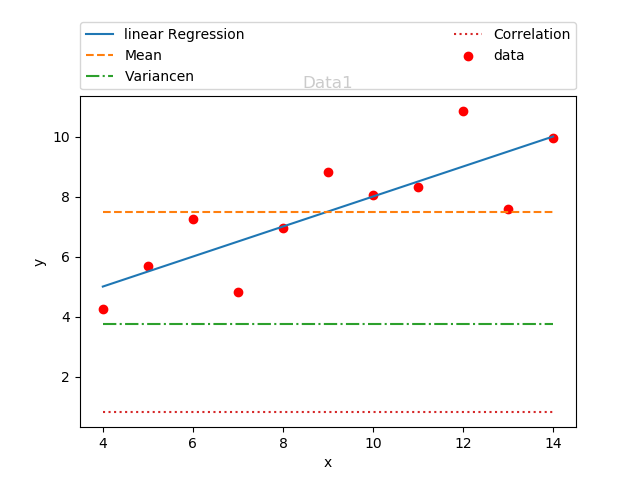
\includegraphics[width=0.7\linewidth]{Data1}
		\caption{Data1}
		\label{fig:data1}
	\end{figure}
	\begin{figure}[!ht]
		\centering
		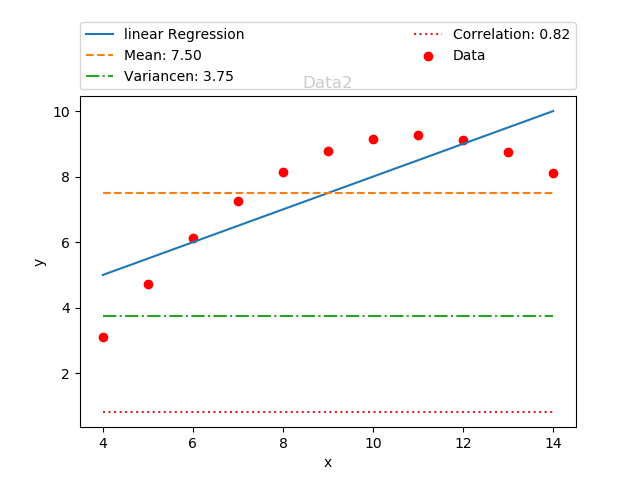
\includegraphics[width=0.7\linewidth]{Data2}
		\caption{Data2}
		\label{fig:data1}
	\end{figure}
	\begin{figure}[!ht]
		\centering
		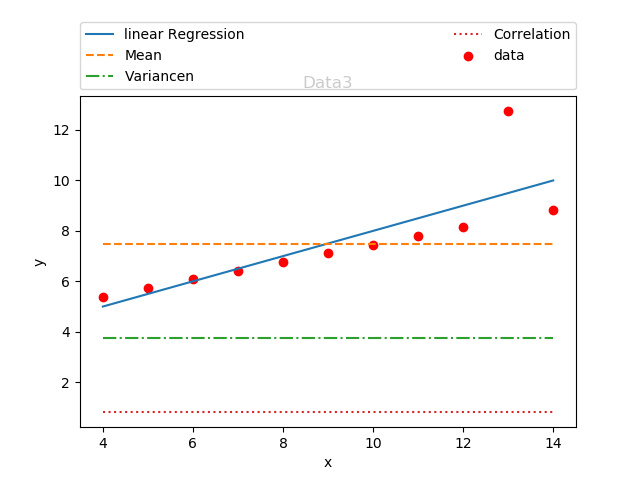
\includegraphics[width=0.7\linewidth]{Data3}
		\caption{Data3}
		\label{fig:data1}
	\end{figure}
	\begin{figure}[!ht]
		\centering
		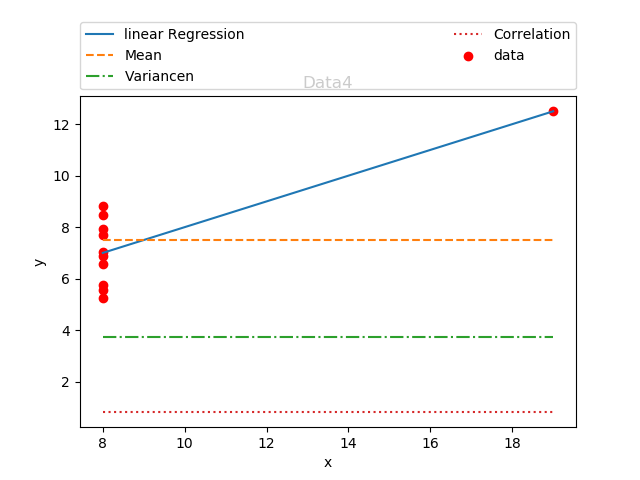
\includegraphics[width=0.7\linewidth]{Data4}
		\caption{Data4}
		\label{fig:data1}
	\end{figure}
	
\end{document}
